\section{Esecuzione}

La prima operazione da noi fatta è stata quella di mettere in moto l'impianto da vuoto portando la camera a una pressione attorno a $10^{-3}$ \si{\pascal}, attorno al vuoto limite del nostro impianto. Abbiamo usato il vacuometro a catodo freddo per controllare il raggiungimento del vuoto limite.

In seguito abbiamo isolato la camera da vuoto chiudendo la valvola gate dalla turbomolecolare. Quindi è stato misurato, tramite il vacuometro pirani connesso alla camera, l'andamento della pressione interna con la valvola a spillo completamente chiusa. Ciò è necessario per misurare la variazione della pressione in camera nel tempo, che in queste condizioni, è dovuta ai soli effetti di degasamento. Questa misura è utile poiché nelle misure successive, volendo ricavare solo il flusso relativo alla valvola a spillo, è opportuno eliminare il contributo dovuto al degasamento. 

Una volta eseguita questa prima serie di misure abbiamo riportato la camera ad una pressione interna di circa $10^{-3}$ \si{\pascal}. Per ogni valore di apertura della valvola, al fine di misurare il flusso in entrata, abbiamo osservato la seguente procedura:
\begin{itemize}
	\item{Si è portata la camera da vuoto\footnote{La valvola a spillo comprende una valvola ausiliaria posta in serie
	alla valvola a vite micrometrica. Tra le due valvole è presente un volume morto, che, se si chiude la valvola ausiliaria
	durante il pompaggio, contiene gas a pressione atmosferica. L'effetto di questo volume di gas, se ignorato, renderebbe
	scorrette le misure. Per ovviare a questo problema abbiamo chiuso la valvola con un tappo e un O-ring in viton e abbiamo
	lasciato aperta la valvola ausiliaria, in modo tale da rendere il volume morto parte della camera e quindi avere ovunque
	la stessa pressione misurata dal vacuometro a catodo freddo.} ad una pressione di circa $10^{-3}$ \si{\pascal},
	controllando con il vacuometro a catodo freddo di essere ad una pressione minore del fondoscala del vacuometro Pirani;}
	\item{È stato spento il vacuometro a catodo freddo per evitare l'usura o il deterioramento dello stesso a causa dell'aumento di pressione.
	In pratica tale sensore è stato usato solo per vedere se si era giunti a pressione limite, quando la pressione era scesa sotto
	il fondoscala del pirani;}
	\item{Si è isolata la camera da vuoto, chiudendo la valvola gate, e la valvola a spillo è stata aperta del numero di giri voluto;}
	\item{È stato tolto il tappo posto a chiusura della valvola a spillo. Si è poi misurato, tramite il multimetro e il sistema di acquisizione dati, il variare della pressione interna della camera in funzione del tempo;}
	\item{Infine la camera da vuoto è stata riportata ad una pressione dell'ordine $10^{-3}$ \si{\pascal}. Nel caso in cui le pressioni
	in camera avessero superato qualche \si{\Pa} di pressione, è stata usata prima la rotativa tramite il bypass, e poi la turbomolecolare.
	Nel caso la pressione finale fosse inferiore al Pascal, abbiamo usato direttamente la turbomolecolare;}
\end{itemize}

Come già detto la prima serie di misure è stata fatta con la valvola a spillo completamente chiusa, per misurare il degasamento.
Le misure successive sono servite ad ottenere i dati di flusso per un'apertura della valvola da 1 a 9 giri della vite micrometrica.
Inoltre è stato misurato l'andamento della pressione nel tempo per aperture di 5.2, 5.4, 5.6 e 5.8 giri.

Grazie alle condizioni meteorologiche stabili, l'intera esperienza è stata svolta in laboratorio ad una temperatura ambiente di $294 \pm 0.5$ \si{\kelvin}, una pressione atmosferica di $981 \pm 0.5$ hPa ed una umidità del $55 \pm 0.5$ \%. Le incertezze di queste ultimi dati sono di risoluzione.

\begin{figure}[h!]
    \centering
    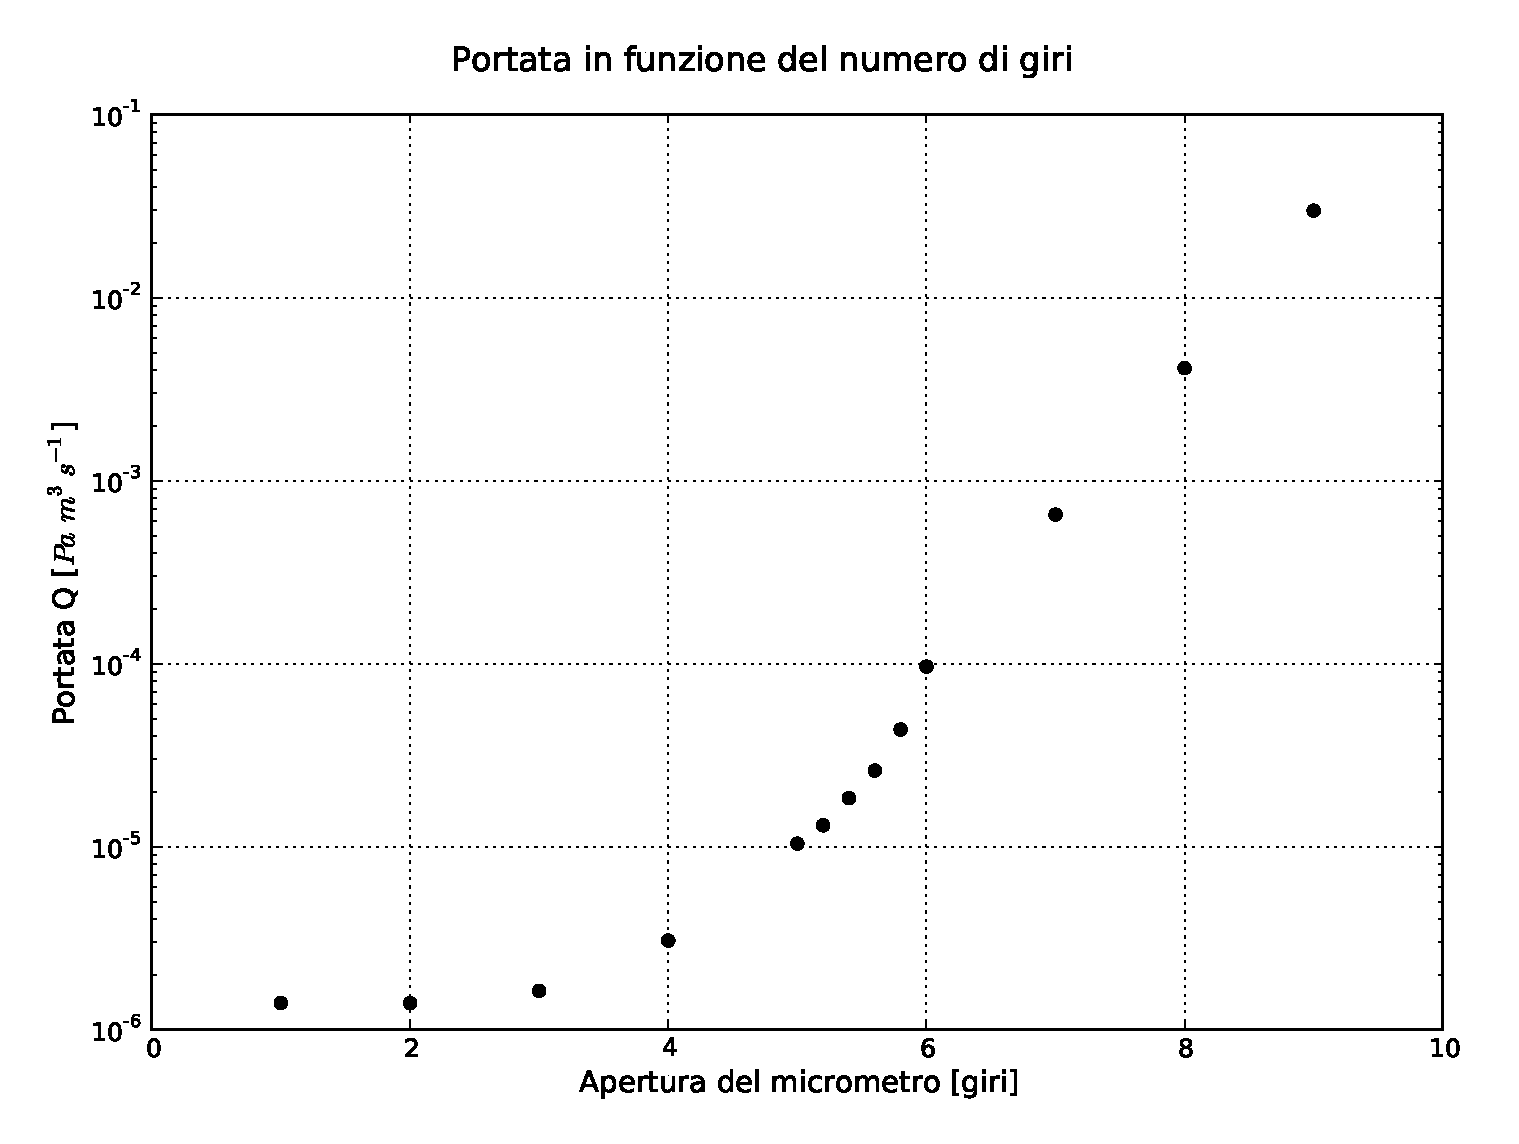
\includegraphics[width=14cm]{graph.pdf}
    \caption{Il grafico mostra i valori elaborati del flusso in entrata a seconda dell'apertura della valvola a spillo. Le barre d'errore non sono
    mostrate in quanto comparabili con la dimensione dei punti sul grafico. L'asse delle ordinate ha scala logaritmica.}
    \label{fig:graph}
\end{figure}

\section{Analisi dati}

Con la procedura descritta sopra, per ogni valore di apertura è stata ottenuta una serie di dati di pressione.
Gli andamenti ottenuti erano in buona approssimazione lineari, come ci si può aspettare, poiché i flussi in ingresso erano costanti.
Abbiamo registrato un andamento lineare anche nel caso della misura del degasamento.
Dai dati abbiamo ricavato, con il metodo della regressione lineare, il valore $\frac{dP}{dt}$ di pendenza di ogni serie di dati.
Grazie a questi dati si può ottenere una stima del flusso in entrata grazie alla seguente relazione:

\begin{equation}
	Q_{tot} \,\, = \,\, V \frac{dP}{dt}
\end{equation}

Bisogna prestare attenzione che il flusso $Q_{tot}$ nella precedente equazione rappresenta il contributo di due differenti fattori: uno è dovuto alla perdita controllata di gas da parte della valvola a spillo, che indicheremo con $Q_{valve}$, mentre il secondo è opera degli effetti di degasamento della camera da vuoto, delle altre parti dell'impianto e di eventuali perdite. Indicheremo questo secondo contributo con $Q_{deg}$.

Pertanto, per ricavare il valore Q$_{valve}$ che ci interessa, occorre sottrarre al flusso totale il flusso dovuto al degasamento:

\begin{equation}
	Q_{valve} \, = \, Q_{tot} \, - \, Q_{deg} \, = \, V \left[ \frac{dP}{dt} - \left(\frac{dP}{dt}\right)_{deg} \right]
\end{equation}

I risultati numerici ottenuti con questa formula, sono visibili nella Tabella \ref{tab:table}.

\begin{table}
    \begin{tabular}{l c c c c c c}
        \toprule
        Nr. giri &
        $Q  [\si{\Pa\cubic\meter\per\second}]$ & $\sigma (Q) [\si{\Pa\cubic\meter\per\second}]$ &
        $S\ped{rotativa} [\si{\cubic\meter\per\second}]$ & $\sigma (S\ped{rotativa}) [\si{\cubic\meter\per\second}]$ &
        $S\ped{turbo} [\si{\cubic\meter\per\second}]$ & $\sigma (S\ped{turbo}) [\si{\cubic\meter\per\second}]$ \\
        \midrule
        1   & 0.00013 & 1.8617e-06 &                   &                   & 0.029125        & 0.00293821154865 \\
        2   & 0.00013 & 1.962e-06  &                   &                   & 0.02879375      & 0.00290824293227 \\
        3   & 0.00016 & 2.2002e-06 &                   &                   & 0.032572        & 0.00328678977752 \\
        4   & 0.00030 & 2.7229e-06 & 0.000131855016235 & 1.32373703717e-05 & 0.03608         & 0.00362219304695 \\
        5   & 0.00103 & 1.3016e-05 & 0.000315597117771 & 3.18067226996e-05 & 0.0399346153846 & 0.00402471748356 \\
        5.2 & 0.00130 & 8.3042e-06 & 0.000351827594516 & 3.52537345308e-05 & 0.040834375     & 0.00409167512276 \\
        5.4 & 0.00184 & 1.1322e-05 & 0.000413355664841 & 4.14134836725e-05 & 0.0438833333333 & 0.00439660530404 \\
        5.6 & 0.00260 & 1.6312e-05 & 0.000478897721927 & 4.79837415967e-05 & 0.04732         & 0.00474128513959 \\
        5.8 & 0.00436 & 2.6838e-05 & 0.000592110619957 & 5.93229678244e-05 & 0.04848         & 0.00485716246794 \\
        6   & 0.00962 & 0.00012289 & 0.000764887079965 & 7.71090559735e-05 & 0.0458547619048 & 0.00462266587445 \\
        7   & 0.06517 & 0.00055883 & 0.00135131654975  & 0.000135627555918 &  & \\
        8   & 0.41163 & 0.0056583  & 0.00176213082573  & 0.000177870106921 &  & \\
        9   & 2.9884  & 0.067334   & 0.00178338842667  & 0.000182809766946 &  & \\
        \bottomrule
    \end{tabular}
\end{table}













































La Tabella \ref{tab:table} ed il relativo grafico in Figura \ref{fig:graph} mostrano chiaramente che l'andamento del flusso non è lineare con
l'apertura della valvola, anzi gli ultimi punti del grafico sembrano suggerire un andamento esponenziale (che su un grafico
con scala logaritmica come quello riportato in figura, risulta in una linea retta). Tuttavia i primi 2/3
punti deviano in maniera vistosa da tale andamento. Da notare inoltre come il flusso di degasamento sia trascurabile
anche per valori piccoli di apertura della valvola.

Abbiamo quindi ricavato il flusso dovuto alla valvola a spillo per alcuni valori di apertura. Questi dati sul flusso ci saranno utili nelle prossime relazioni.
